\apendice{Planificación}

\section{Introducción}
En las primeras semanas, de manera previa a utilizar cualquier metodología de desarrollo software, debemos de probar distintas aproximaciones a nuestro problema. Para que finalmente podamos escoger la más adecuada entre las distintas posibilidades.

Aunque no se aplique una metodología ágil, se asignarán unas tareas semanales para llevar a cabo la traceabilidad del desarrollo del proyecto, así como el control del estudio sobre la problemática a realizar durante cada semana o \textit{milestone}.

Una vez escogida la mejor solución posible comenzaremos a utilizar una metodología ágil de desarrollo.

\section{Estudio previo}

\subsection{Semana 0}
Estas son las tareas a realizar durante esta semana 0:

\begin{itemize}
	\item Probar LaTeX
	\item Gestor de tareas/versiones: Github y Zenhub
	\item Instalar anaconda y Jupyter
	\item Leer los artículos propuestos por los tutores
	\item Comenzar a probar algunos algoritmos de binarización
\end{itemize}

Como se puede ver las tareas a realizar son triviales puesto que es la semana 0 y es una semana de mera adaptación al entorno de trabajo. La única tarea que supone un esfuerzo de comprensión mayor es la lectura de los artículos propuestos sobre trabajos relacionados o con una problemática similar a la nuestra. A continuación en la figura \ref{fig:A.1.1} se muestra el diagrama \textit{burndown} de esta semana. 

\begin{figure}[h]
\centering
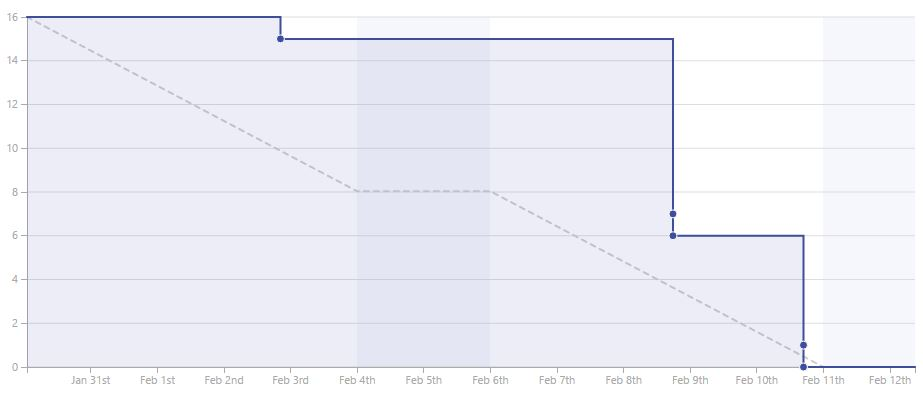
\includegraphics[width=0.99\textwidth]{semana_0}
\caption{Burndown de la semana 0}
\label{fig:A.1.1}
\end{figure}

\subsection{Semana 1}
Estas son las tareas a realizar durante esta semana 1:

\begin{itemize}
	\item Documentar lo realizado durante la semana 0
	\item Documentar lo que se irá realizando durante esta semana 1
	\item Continuar probando con algoritmos de procesamiento de imágenes
	\item Probar una aproximación con clasificadores al problema
\end{itemize}

Puesto que en la semana anterior no se documento lo realizado, durante esta semana se pretende documentar todo lo realizado durante la semana anterior y esta semana. Además de continuar probando con algoritmos de procesamiento de imágenes y comenzar a probar con la aproximación al problema mediante clasificadores.

En esta semana me vi desbordado de trabajo debido a la subestimación del esfuerzo a empeñar en las distintas tareas. No siendo capaz de comenzar a probar una aproximación con clasificadores.

\begin{comment}
\begin{figure}[h]
\centering
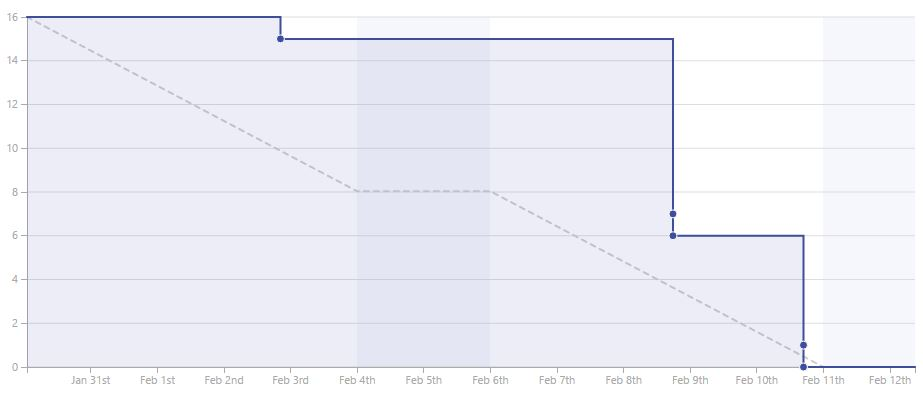
\includegraphics[width=0.99\textwidth]{semana_0}
\caption{Burndown de la semana 0}
\label{fig:A.1.1}
\end{figure}
\end{comment}


\section{Planificación temporal}

\section{Estudio de viabilidad}

\subsection{Viabilidad económica}

\subsection{Viabilidad legal}


